\documentclass[a5paper]{article}
% Uncomment the following line to allow the usage of graphics (.png, .jpg)
%\usepackage[pdftex]{graphicx}
% Comment the following line to NOT allow the usage of umlauts

\pagestyle{empty}
\usepackage[T2A]{fontenc}
\usepackage[utf8]{inputenc}
\usepackage[russian]{babel}
\usepackage{cmap}
\usepackage{amsthm}
\usepackage{amsmath}
\usepackage{units}
\usepackage{fancyhdr}
\usepackage{forloop}
\usepackage{amssymb}
\usepackage{url}
\usepackage{hyperref}
\usepackage{xcolor}
\usepackage[inline]{enumitem}
\usepackage{graphicx}
\usepackage{epstopdf}

\usepackage{caption}
\usepackage{subcaption}
\usepackage{amscd}

\def \topic {Семинар 1}

\renewcommand{\thesection}{\arabic{section}}

\renewcommand{\headrulewidth}{0.4pt}
\renewcommand{\footrulewidth}{0.4pt}

\fancyfoot[C]{\thepage}
\fancyfoot[L]{}

\fancyhead[R]{\thepage}
%For multipage documents only!
%\fancyfoot[L]{page: \thepage}
\fancyhead[L]{Перечислительная комбинаторика}
\fancyfoot[C]{\topic}

\pagestyle{fancy}

\renewcommand{\baselinestretch}{1.0}
\renewcommand\normalsize{\sloppypar}

\setlength{\topmargin}{-0.5in}
\setlength{\textheight}{6.5in}
\setlength{\oddsidemargin}{-0.3in}
\setlength{\evensidemargin}{-0.3in}
\setlength{\textwidth}{4.5in}
\setlength{\parindent}{0ex}

\newcounter{problemset}
\newcounter{totalpages}
%Here you should set the total number of pages
\setcounter{totalpages}{1}

\def \Z {\mathbb Z}
\def \R {\mathbb R}
\def \P {\mathbb P}
\def \C {\mathbb C}
\def \vec {\boldsymbol}

\theoremstyle{definition}
\newtheorem{lemma}{Лемма}
\newtheorem{example}{Пример}
\newtheorem*{theorem}{Теорема}
\newtheorem*{definition}{Определение}

\makeatletter
\renewcommand{\section}{\@startsection
{section}%                   % the name
{1}%                         % the level
{\z@}%                       % the indent / 0mm
{-\baselineskip}%            % the before skip / -3.5ex \@plus -1ex \@minus 
%%-.2ex
{0.5\baselineskip}%          % the after skip / 2.3ex \@plus .2ex
{\centering\large\scshape}} % the style

\renewcommand{\subsection}{\@startsection
{subsection}%                % the name
{1}%                         % the level
{\z@}%                       % the indent / 0mm
{-\baselineskip}%            % the before skip / -3.5ex \@plus -1ex \@minus 
%%-.2ex
{0.5\baselineskip}%          % the after skip / 2.3ex \@plus .2ex
{\centering\large\scshape}} % the style
\makeatother


\begin{document}

\begin{center}

\newcommand{\HRule}{\rule{\linewidth}{0.5mm}}
\HRule \\[0.2cm]
{ \Large \bfseries \topic} %\\[0.2cm]
\HRule

\end{center}

\section{Производящие функции. Тизер}

Среди читателей этого документа и слушателей курса, как мне кажется, могут 
оказаться люди, которые уже слушали в моём изложении элементы этой теории, 
впрочем, я всё-таки буду ориентироваться в основном на тех, кто будет видеть 
этот курс впервые.
О производящих функциях я рассказывал много, ещё с девятого класса, начиналось 
это с замысловатых <<олимпиадных задачек>>, каждая из которых была сама по себе 
красива, но было совсем непонятно, какая общая концепция может за этим стоять 
(кроме мистического словосочетания <<производящая функция>>). Приведу несколько 
примеров.

\begin{enumerate}
	\item (IMO Shortlist-2007). Элементы множества \( S = \{1,2,\ldots, n\} \) 
	покрашены в синий и красный цвет, причём синих и красных элементов \( r \) 
	и \( b \) штук соответственно. Оказалось, что среди троек элементов \( S 
	\times S \times S \) есть ровно \( 2007 \) таких троек \( (x,y,z) \), что 
	одновременно выполнены два условия
	\begin{enumerate}
		\item \( x,y, z \) одного цвета
		\item \( x  + y + z \) делится на \(  n \).
	\end{enumerate}
	Докажите, что \( r^2 + rb + b^2 = 2007 \).
	
	Решение: рассмотрим многочлен \( F(x) = x^{a_1} + x^{a_2} + \ldots + 
	x^{a_r} \), где \( a_i \)~--- шары красного цвета...
	\item (IMO Shortlist-1998). Пусть \( a_0, a_1, a_2, \ldots \)~--- 
	возрастающая последовательность 
	целых неотрицательных чисел, такая, что любое целое неотрицательное число 
	может быть единственным образом представлено в виде \( a_i + 2a_j + 4 a_k 
	\), где \( i,j,k \) не обязательно различны. Найдите \( a_{2017} \).
	
	Решение: рассмотрим многочлен \( x^{a_0} + x^{a_1} + \ldots \)...
	\item Пусть \( n \)~--- натуральное число. Найдите количество таких 
	многочленов \( P(x) \) с коэффициентами из множества \( \{0,1,2,3\} \), что 
	\( P(2) = n \).
	
	Решение: пусть количество таких многочленов равно  \( q_n \). Рассмотрим 
	многочлен \( Q(x) = q_0 + q_1 x + q_2 x^2 + \ldots \).
	\item {}[[ Здесь могла быть задача про перечисление сакур. ]]
\end{enumerate}

Чем больше я про это рассказывал, тем больше узнавал нового для себя, читая 
разную литературу. Три года назад я нашёл лекции Седжвика и Флажоле \cite{ac} 
на сайте \texttt{coursera.org}, и сразу понял: вот оно! Я наконец стал понимать 
структуру, которая стоит за такими задачами. Любая задача на перечисление 
объектов, если она \textit{правильно} сформулирована, может быть решена.

Область применений этой техники поистине внушительна: многочлены, отображения, 
графы, разбиения, задачи на строки, анализ алгоритмов, и так далее. Несколько 
примеров задач из книги \cite{ac} и другой литературы, но уже более 
<<наукообразных>>.

\begin{enumerate}
	\item Количество способов представить число \( n \) в виде суммы 
	натуральных слагаемых \( n = s_1 + s_2 + \ldots + s_k \) (не обязательно 
	различных, \( k \) не фиксировано) равно \( 2^{n-1} \).
	
	Подсказка: производящая функция таких разбиений имеет вид
	\[
		C(z) = \dfrac{1}{1 - \dfrac{1}{1-z}} = \dfrac{1-z}{1 - 2z}
		\enspace .
	\]
	Этот пример мы детально рассмотрим в следующем параграфе.
	\item Количество \textit{циклических разбиений} числа \( n \) на \( k \) 
	слагаемых (то есть скажем, разбиение \( 2 + 3 + 1 + 2 + 5 \) не отличается 
	от разбиения \( 3 + 1 + 2 + 5 + 2 \)) имеет асимптотический рост \( \sim 
	\dfrac{n^{k-1}}{(k-1)!} \). Здесь \( k \) фиксировано, а \( n \)  растёт.
	
	Кстати, методы аналитической комбинаторики позволяют не только получать 
	асимптотический рост в смысле <<главной асимптотики>>, но и часто получать 
	полное 
	асимптотическое разложение коэффициентов, и эти формулы можно использовать 
	в дальнейшем для практических вычислений, если взять достаточное количество 
	членов разложения. (Да-да, эта наука иногда даже используется на практике).
	\item Количество разбиений \( n \) на \textit{различные} слагаемые не 
	выражается в явном виде \cite[section VIII.6, p.574]{ac}, но имеет 
	асимптотику
	\[
		Q_n \sim \dfrac{3^{3/4}}{12 n^{3/4}} \exp \left( \pi \sqrt{\dfrac n 3} 
		\right)
	\]
	
	Комментарий: эта асимптотика выглядит пугающе, неизвестно откуда взявшиеся 
	степени \( 3/4 \), и самое главное, число пи в экспоненте. Но мы увидим, 
	что этот результат~--- всего лишь рутинное применение техник из ТФКП.
	
	\item Обозначим \( {n \choose k}_{<d} \) число \( k \)-элементных <<не 
	разреженных>> подмножеств множества \( \{1,2,\ldots, n\} \), то есть таких, 
	что никакой элемент не может быть на расстоянии \( d \) или более от 
	следующего за ним по возрастанию (если \( a_1 < a_2 < \ldots < a_k \), то 
	\( a_{j+1} - a_j < d \)). Тогда выполнено
	\[
		{n \choose k}_{<d} = \sum_j (-1)^j {k-1 \choose j}{n - dj \choose k}
	\]
	Это следует из формулы
	\[
		\sum_{n \geq 0} {n \choose k}_{<d} z^n = \dfrac{z^k 
		(1-z^d)^{k-1}}{(1-z)^{k+1}}.
	\]
	\item Десятки задач по теории кодирования \cite[Section I.4, I.24, p. 
	53]{ac}, регулярным языкам и автоматам, обобщениям чисел Каталана для 
	деревьев разной формы \cite[Section I.5]{ac}, разложениям на множители 
	полиномов над конечными полями \cite[Example VII.4, p. 449]{ac}, 
	перечисление лямбда-термов \cite{lambda}, перечисление графов на 
	поверхностях \cite{graphs_manifolds}, всего и не \textit{перечислишь}.
	\item\( ^{\ast} \) Вот пример того, как проявляется комбинаторная природа 
	элементарных функций:
	\begin{enumerate}
	\item Любая перестановка \( n \) элементов представляется в виде множества 
	циклов: \textsc{Perm}=\textsc{Set}\( \circ \)\textsc{Cyc}.
	\item Экспонента и логарифм являются взаимно обратными функциями:
	\[
		\exp\left(\log \dfrac{1}{1 - x}\right) = \dfrac{1}{1 - x}
	\]
	\end{enumerate}
	Вот ещё пара примеров на ту же тему. Экспоненциальная производящая функция 
	для пилообразных перестановок нечётной длины равна \( \tan x \), а чётной 
	\( \dfrac{1}{\cos x} \). Здесь начинается так называемая 
	\textit{комбинаторная тригонометрия}: можно дать \textit{комбинаторное 
	доказательство} некоторых тригонометрических тождеств \cite[Exercise 5.7, 
	p. 74]{stanley2}
	\begin{enumerate}
		\item \( 1 + \tan^2 x = \dfrac{1}{\cos^2 x} \),
		\item \( \tan(x + y) = \dfrac{\tan x + \tan y}{1 - \tan x \tan y} \)
	\end{enumerate}
	Экспоненциальная производящая функция для полиномов Лаггера имеет вид
	\[
		\sum_{n \geq 0}\mathcal L^{(\alpha)}_{n}(t) \dfrac{x^n}{n!} = 
		\left(\dfrac{1}{1 - x}\right)^{\alpha + 1} \exp\left(
			\dfrac{-tx}{1 - x}
		\right) \enspace .
	\]
	Это тождество предполагает комбинаторную природу этих полиномов, которая 
	состоит из перестановок (имеющих \( \alpha + 1 \) циклов) и ориентированных 
	цепей (каждая с весом \( -t \)). Различные тождества для полиномов Лаггера 
	могут быть получены как элементарные конструкции для дискретных структур. 
	Книга Theory of Species
	\cite{species} содержит комбинаторное описание разных семейств полиномов 
	(Эйлер, Эрмит, Лаггер, Якоби) и 
	ссылки на соответствующую литературу (многие из этих полиномов встретятся в 
	стандартном курсе физтеха, но в контексте теоретической физики и уравнений 
	матфизики).
\end{enumerate}

Я попробую начать своё изложение совсем в другом ключе, не так, как я это делал 
раньше. Сейчас мы узнаем некоторые элементы <<theory of species>>, теории, по 
которой была написана книга \cite{species} в 1998 году, а затем я постараюсь 
дать обзор методов перечислительной комбинаторики из книги Флажоле и Седжвика 
\cite{ac}: как от комбинаторных конструкций мы строим производящие функции и 
приходим к дифференциальным уравнениям, и как потом анализировать асимптотику 
роста коэффициентов из этих дифференциальных уравнений.

\section{Помеченные и непомеченные объекты}

Перед тем, как творить магию, давайте немного позанимаемся формализмом.

\begin{definition}
	\textit{Объект} \( A \) представляет из себя пару \( (U, \gamma) \), где \( 
	U \)~--- множество первых нескольких натуральных чисел \( U = \{1, 2, 
	\ldots, n\} \) для некоторого \( n \), а \( \gamma \)~--- некая 
	теоретико-множественная\footnote{Мы не будем формально определять, что 
	такое теоретико-множественная структура, как не будем определять, что такое 
	множество. В книге \cite{species} авторы избегают эту проблему, исследуя 
	поведение классов при действии перестановок, а также накладывая некоторые 
	\textit{функториальные ограничения} на классы объектов. Стоит ли лезть в 
	такие дебри, или нет, вопрос спорный, мы же сосредоточимся на других 
	моментах.} структура на \( U \).
\end{definition}

\begin{figure}[h]
\centering
\begin{subfigure}{.22\textwidth}
   	\centering
	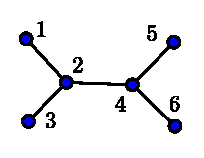
\includegraphics[width=.5\textwidth]{planar_nonrooted.eps}
	\caption{Планарное дерево}
	\label{fig:planar_1}	
\end{subfigure}%
\begin{subfigure}{.22\textwidth}
	\centering
	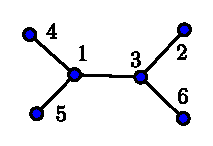
\includegraphics[width=.5\textwidth]{planar_nonrooted_2.eps}
	\caption{Изоморфное дерево}
	\label{fig:planar_2}	
\end{subfigure}%
\begin{subfigure}{.22\textwidth}
	\centering
	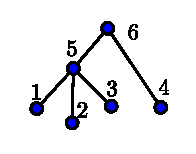
\includegraphics[width=.5\textwidth]{planar_nonrooted_3.eps}
	\caption{Другое дерево}
	\label{fig:planar_3}	
\end{subfigure}%
\begin{subfigure}{.22\textwidth}
	\centering
	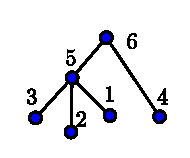
\includegraphics[width=.5\textwidth]{planar_nonrooted_4.eps}
	\caption{Ещё одно дерево}
	\label{fig:planar_4}	
\end{subfigure}
\caption{Дерево как частный случай произвольного графа}
\end{figure}

\begin{example}
Давайте считать, что \textit{граф}~--- это набор вершин \( U \), а структура \( 
\gamma \) является \textit{множеством} \textit{рёбер}, где, в свою очередь, 
каждое ребро это множество из двух вершин. Тогда на рисунках 
\ref{fig:planar_1}, \ref{fig:planar_2}, \ref{fig:planar_3} изображены, 
соответственно, деревья
\begin{eqnarray*}
	(\{1,2,3,4,5,6\}, \{ \{1,2\}, \{2,3\}, \{2,4\}, \{4,5\}, \{4,6\} \}), \\
	(\{1,2,3,4,5,6\}, \{ \{1,4\}, \{1,5\}, \{1,3\}, \{2,3\}, \{3,6\} \}), \\
	(\{1,2,3,4,5,6\}, \{ \{1,5\}, \{2,5\}, \{3,5\}, \{5,6\}, \{4,6\} \}), \\
	(\{1,2,3,4,5,6\}, \{ \{3,5\}, \{2,5\}, \{1,5\}, \{5,6\}, \{4,6\} \}).
\end{eqnarray*}
Если бы мы решили в качестве ребра рассматривать не множество, а пару вершин, 
получился бы \textit{ориентированный граф}.
\end{example}

Что стоит за словами \textit{помеченный} и \textit{непомеченный} объект? Для 
того, чтобы говорить о помеченных и непомеченных объектов, нужно сказать, какие 
объекты мы считаем различными, а какие одинаковыми, и в каком контексте.

На рисунках \ref{fig:planar_3}, \ref{fig:planar_4} изображено одно и то же 
дерево, потому что структуры \( \gamma \) для этих деревьев одинаковые. На 
рисунках 
\ref{fig:planar_1} и \ref{fig:planar_2} изображены разные деревья. Будем 
говорить, что объекты \( A \), \( B \) \textit{совпадают}, если соответствующие 
структуры \( \gamma_A \), \( \gamma_B \) тоже совпадают. С точки зрения нашего 
жаргона, 
\( A \) и \( B \) задают одну и ту же \textit{помеченную структуру}, потому что 
вершины помечены натуральными числами (цветами) от \( 1 \) до \( 6 \).

Будем говорить, что объекты \( A \) и \( B \) \textit{изоморфны}, если 
существует перестановка элементов \( \sigma \colon U_A \to U_B \), такая, что 
естественный транспорт \( \gamma_A \to \sigma(\gamma_A) \) совпадает с \( 
\gamma_B \). В данном случае деревья на рисунках \ref{fig:planar_1} и 
\ref{fig:planar_2} \textit{изоморфны}, потому что существует перестановка 
элементов, такая, что соответствующая структура \( \gamma_A \) перейдёт в 
структуру \( \gamma_B \). Деревья на рисунках \ref{fig:planar_1} и 
\ref{fig:planar_3} не являются изоморфными (подумайте, почему). На нашем 
жаргоне изоморфные структуры задают один и тот же \textit{непомеченный} объект.

Элементы множества \( U \) иногда называют \textit{атомами} или \( s 
\)-\textit{объектами}. Таким образом, каждый \textit{объект} состоит из 
\textit{атомов}, а объекты, как мы скажем позже, объединяются в \textit{классы 
объектов} (например, класс всевозможных помеченных деревьев, класс всех строк в 
бинарном алфавите, и так далее).

Перед тем, как переходить к производящим функциям, полезно 
поставить ещё один мысленный эксперимент. Корневые (подвешенные) деревья 
допускают два различных описания в виде структур. Первое описание --- в виде 
графа (без циклов) с выделенной вершиной. Второе описание --- как множество \( 
\{ r, T_1, \ldots \} \), где \( r \in U \)~--- номер вершины-корня дерева, а \( 
T_k \)~--- множества, соответствующие поддеревьям.

	\begin{figure}[h]
	\centering
    \begin{subfigure}{.5\textwidth}
    	\centering
		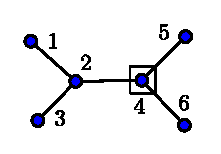
\includegraphics[width=.5\textwidth]{structure_isomorphism_1.eps}
		\caption{Описание в виде графа}
		\label{fig:iso_1}	
	\end{subfigure}%
    \begin{subfigure}{.34\textwidth}
		\centering
		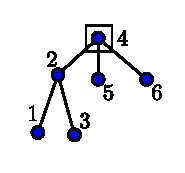
\includegraphics[width=.5\textwidth]{structure_isomorphism_2.eps}
		\caption{Описание в виде дерева}
		\label{fig:iso_2}	
	\end{subfigure}%
    \end{figure}

Эти описания можно выразить в виде
\begin{eqnarray*}
	\gamma_{(1)} &=& (
		\{ 4 \}, \{ \{ 1,2 \}, \{2,3\}, \{2,4\}, \{4,5\}, \{4,6\} \}
	) \enspace ,\\
	\gamma_{(2)} &=& \{
		4, \{5\}, \{6\}, \{
			2, \{1\}, \{3\}
		\}
	\} \enspace .
\end{eqnarray*}

Если эти описания оторваны от контекста (то есть от множества всех подвешенных 
корневых деревьев), то бессмысленно говорить о том, что они задают одно и то же 
дерево. Пусть задан \textit{класс объектов} \( \mathcal A \). Каждый объект \( 
a \in \mathcal A \) имеет вид \( (U, \gamma) \), и разным объектам могут 
соответствовать разные \( U \). Тогда можно говорить об \textit{изоморфизме} 
классов объектов.

Если существует \textit{биекция} из класса объектов \( \mathcal A \) в класс 
объектов \( \mathcal B \), \( F \colon \mathcal A \to \mathcal B \) которая 
сохраняет размер объекта (мощность множества \( U \)):
\[
	F(U, \gamma) = (V, \eta), \quad |U| = |V|
\]
то говорят, что классы объектов \( \mathcal A \) и \( \mathcal B \) 
\textit{эквипотенциальны}. 
В книге \cite{gouldenjackson} говорят, что класс \( \mathcal B \) задаёт 
\textit{представление} класса \( \mathcal A \). Если говорить по-русски, то 
классы \textit{эквипотенциальны}, если количество помеченных объектов размера 
\( n \) одинаковое в обоих классах для каждого \( n \).

Понятие эквипотенциальности не совсем хорошо подходит для описания изоморфизма 
классов объектов. Ниже мы рассмотрим примеры, которые это подтверждают. Значит, 
нам нужно другое определение.
На этом вопросе хочется задержаться подольше, потому что если об этом не 
задуматься, то задумываться потом будет уже поздно. Но я призываю читателя 
потерпеть, и ближе к концу лекции мы постараемся залатать эту брешь в 
фундаменте.

\section{OGF. Обыкновенные производящие функции}

\begin{example}[{\cite[Example 10, p.36]{species}}]
Бюллетень для голосований устроен следующим образом: имеется несколько 
кандидатов, и необходимо раздать этим кандидатам предпочтения, не обязательно 
различные. Сначала отмечается 
непустое множество наиболее предпочтительных кандидатов (уровень 1), затем 
непустое множество следующих по предпочтению (уровень 2), и так, 
пока всем кандидатам не будут назначены предпочтения. Пропускать уровни нельзя. 
Сколько 
существует способов заполнить бюллетень, в котором всего \( n \) кандидатов? 

Заметим, что если считать кандидатов различимыми, то кандидатам можно 
сопоставить натуральные числа \( \{1, 2, \ldots, n\} \). Каждый уровень будет 
представлять собой подмножество \( \{1,2,\ldots, n\} \), и таким образом 
каждый бюллетень является помеченным объектом. Если кандидаты 
неразличимы (нас интересует только количество выбранных кандидатов на каждом 
уровне), то это множество непомеченных объектов.

Для начала мы рассмотрим ситуацию, когда кандидаты неразличимы. 

	\begin{figure}[h]
	\centering
    \begin{subfigure}{.5\textwidth}
    	\centering
		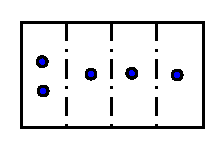
\includegraphics[width=.5\textwidth]{ballots_1.eps}
		\caption{Непомеченные: OGF}
		\label{fig:unrooted_trees}	
	\end{subfigure}%
    \begin{subfigure}{.5\textwidth}
		\centering
		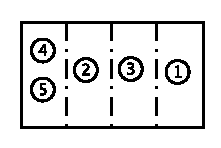
\includegraphics[width=.5\textwidth]{ballots_2.eps}
		\caption{Помеченные: EGF}
		\label{fig:cycle_unrooted}	
	\end{subfigure}%
    \end{figure}


Стратегия решения этой задачи будет следующей: пусть существует \( b_n \) 
способов заполнить бюллетень с \( n \) кандидатами. Тогда мы хотим выразить 
формальный степенной ряд
\[
	B(x) = b_0 + b_1 x + b_2 x^2 + \ldots \enspace ,
\]
с помощью известных нам элементарных функций (синусы, экспоненты, рациональные 
функции, и т.д.), а затем уже найти выражение для коэффициентов \( b_n \). 
Такой формальный степенной ряд называется \textit{производящей функцией}. 
Коэффициент при \( x^n \) обозначает количество \textit{неизоморфных} объектов, 
содержащих \( n \) неразличимых
атомов (или другими словами, количество объектов размера \( n \), с точностью 
до изоморфизма).

Заметим, что каждый уровень представляет собой \textit{непустое множество} 
(\textsc{set}\( ^{+} \)) неразличимых кандидатов, а весь бюллетень~--- 
\textit{последовательность} (\textsc{seq}) уровней. Значит, если обозначить 
неразличимого кандидата символом \( \bullet \), то символически бюллетень 
представляет из себя конструкцию
\[
	\mathrm{Ballot} = \text{\textsc{seq}(\textsc{set$^{+}$}($\bullet$))}
	\enspace .
\]
Попробуем получить формальные степенные ряды для составных частей этой 
конструкции, а затем поймём, какая между ними взаимосвязь.

<<Забудем>> про сложные бюллетени и рассмотрим бюллетень, состоящий из одного 
уровня.

Если количество кандидатов на одном \textit{уровне} равно \( n \geq 1 \), то 
количество таких уровней равно \( 1 \), ведь кандидаты неразличимы. Таким 
образом, \textit{производящая функция} для уровня имеет вид
\[
	\mathrm{Level}(x) = x + x^2 + x^3 + \ldots = \dfrac{x}{1-x} \enspace ,
\]
где коэффициент при \( x^n \)  равен количеству уровней, содержащих \( n \) 
кандидатов. Чтобы перечислить все возможные бюллетени, мы перечислим бюллетени, 
имеющие ровно \( k \) уровней, а затем объединим результат по всем \( k \). 
Если в бюллетене имеется два уровня, то чтобы получить производящую функцию 
таких бюллетеней, необходимо перемножить соответствующие производящие функции:
\[
	\mathrm{Ballot}^{[2]} (x) = \mathrm{Level}(x)^2 = \dfrac{x^2}{(1 - x)^2} 
	\enspace .
\]
Действительно, если такой бюллетень содержит два уровня и \( n \) кандидатов, 
то первый уровень имеет произвольное число \( j \) кандидатов, а второй уровень 
соответственно \( n-j \). Значит, общее число бюллетеней выражается суммой
\[
	\sum_{j=0}^{n} a_j a_{n-j} \enspace ,
\]
где \( a_{j \geq 0} = 1 \), \( a_0 = 0 \)~--- количество уровней, имеющих \( j 
\) кандидатов. Если перемножить два формальных степенных ряда и раскрыть 
скобки, то мы заметим, что
\begin{multline*}
	\left(a_0 + a_1 x + a_2 x^2 + \ldots
    \right)
    (b_0 + b_1 x + b_2 x^2 + \ldots) =\\
     a_0 b_0 
	+ (a_0 b_1 + a_1 b_0) x + (a_0 b_2 + a_1 b_1 + a_2 b_0) x^2 + \ldots
	\enspace ,
\end{multline*}
и коэффициент при \( x^n \) в произведении будет равен \( \sum_{j=0}^{n} a_j 
b_{n-j} \). Мы только что выяснили, что производящая функция для 
\textit{декартова произведения} объектов равна \textit{произведению} 
производящих функций исходных объектов. Это же утверждение верно не только для 
пар, но и для троек, для четвёрок, то есть для конечных последовательностей, 
или \textit{кортежей}
объектов.

Значит, число бюллетеней, которые содержат \( k \) уровней, равно
\[
	\mathrm{Ballot}^{[k]}(x) = \mathrm{Level}(x)^{k} = 
	\left(\dfrac{x}{1-x}\right)^k \enspace .
\]
Любой бюллетень содержит некоторое ненулевое число уровней. Производящая 
функция \textit{непересекающегося объединения} двух множеств равна 
\textit{сумме} производящих функций этих множеств. Другими словами,
\[
	\mathrm{Ballot}(x) = \sum_{k \geq 1} \mathrm{Ballot}^{[k]}(x) = \sum_{k 
	\geq 1} \left(\dfrac{x}{1-x}\right)^k = \dfrac{\dfrac{x}{1-x}}{1 - 
	\dfrac{x}{1 - x}} 
	= \dfrac{x}{1 - 2x}
	\enspace .
\]
Остальное~--- дело техники, нужно лишь представить функцию \( 
\mathrm{Ballot}(x) \) в виде формального степенного ряда, или формулой Тейлора 
в окрестности нуля.
\[
	\dfrac{x}{1 - 2x} = \sum_{n \geq 1} 2^{n-1} 
	x^n \enspace .
\]
Таким образом, количество бюллетеней с \( n \) кандидатами равно \( 2^{n-1} \).
\end{example}

\subsection{OGF. Рефлексируем над примером}

Важность этого примера состоит в том, что он даёт первоначальное понятие о том, 
что такое производящая функция, и рассказывает сразу про два 
комбинаторных оператора, а также про то, как они действует на производящие 
функции. Первый оператор~--- это \textit{непересекающееся объединение}, \( 
\mathcal A 
\sqcup \mathcal B \), и для него есть сумма производящих функций:
\[
	F_{\mathcal A \sqcup \mathcal B}(x) = F_{\mathcal A}(x) + F_{\mathcal B}(x) 
	\enspace .
\]
Слово \textit{непересекающееся} здесь имеет чисто технический характер. Ясно, 
что бюллетень, который содержит три уровня, не может олновременно являться 
юллетенем, содержащим два уровня. (В противоположность базам данных, где 
автобус может являться троллейбусом). Так, например, непересекающееся 
объединение множеств \( \mathbb N \sqcup \mathbb N \) являет собой две копии \( 
\mathbb N \):
\[
	\mathbb N \sqcup \mathbb N \cong
	\{
		1_x, 2_x, 3_x, \ldots,
		1_y, 2_y, 3_y, \ldots
	\}
\]

Второй оператор~--- это \textit{декартово произведение}, \( \mathcal A \times 
\mathcal B \), то 
есть множество пар
\[
	\mathcal A \times \mathcal B = \{ (a, b) \mid a \in \mathcal A, b \in 
	\mathcal B \} \enspace .
\]
Определение, которое написано выше, немного <<наивно>> в том смысле, что в 
начале рассказа мы договорились, что все \textit{объекты} имеют вид \( (U, 
\gamma) \), где \( \gamma \)~--- структура над \( U \), где \( U \), в свою 
очередь, имеет вид \( \{ 1, 2, \ldots, n \} \). На самом деле, идеологически 
правильнее взять два объекта \( a \in \mathcal A \), \( b \in \mathcal B \), 
где атомы объекта \( a \) это \( \{ 1, 2, \ldots, n \} \), а атомы объекта \( b 
\) это \( \{1,2,\ldots, m  \} \). Затем рассмотреть всевозможные объекты, 
построенные на атомах \( \{ 1, 2, \ldots, n+m \} \), имеющие структуру \( 
(\gamma_1, \beta_1) \), где структуры \( \gamma_1, \beta_1 \) наследуются от  
соответствующих структур \( \gamma, \beta \) объектов \( a \) и \( b \), а 
номера атомов присваиваются всеми \( 
C_{n+m}^{n} \) возможными способами. Так как мы рассматриваем 
\textit{непомеченные объекты}, то есть объекты с точностью до изоморфизма, 
атомы для нас неразличимы, и поэтому такое определение на данном этапе немного 
избыточно, рекомендую отложить его до момента, когда мы обратимся к помеченным 
объектам.

Интуитивно всё очень прозрачно. Если \( \mathcal A \), \( \mathcal B \) это 
строки, то объекты из \( \mathcal A \times \mathcal B \) это пары строк. Если 
\( \mathcal A \), \( \mathcal B \) это натуральные числа, то объекты из \( 
\mathcal A \times \mathcal B \) это пары чисел. Здесь уместно представить, что 
натуральное число \( n \) представляется как \( n \) неразличимых атомов. Тогда 
количество атомов в паре \( (n, m) \) равно \( m + n \).

Этому оператору 
соответствует произведение 
производящих функций:
\[
	F_{\mathcal A \times \mathcal B}(x) = F_{\mathcal A}(x) \cdot F_{\mathcal 
	B}(x) \enspace.
\]
Оператор типа <<тройка объектов>> получается последовательным применением 
оператора <<пара объектов>>:
\[
	\mathcal A \times \mathcal B \times \mathcal C = (\mathcal A \times 
	\mathcal B) \times \mathcal C \neq \mathcal A \times (\mathcal B \times 
	\mathcal C) = \mathcal A 
	\times \mathcal B \times \mathcal C
	\enspace .
\]
Выше написана некоторая загадочная противоречивая формула, смысл которой 
состоит в том, что объекты \( (a, (b, c)) \) и \( ((a, b), c) \)~--- это 
формально \textit{два разных объекта}! Это различие в будущем позволит нам 
рассматривать структуры типа деревьев. Широко известный факт: количество 
бинарных деревьев равно количеству правильных скобочных последовательностей. Но 
в данном примере с бюллетелями не имеет значения, какой способ построить тройку 
мы выбрали: производящая функция для тройки объектов всегда будет иметь вид \( 
A(x) \cdot B(x) \cdot C(x) \).

Затем, если объединить все последовательности конечной длины, составленные из 
объектов класса \( \mathcal A \) (в том числе и 
нулевой длины), можно получить новый оператор \textsc{seq}\( (\mathcal A) \), 
который действует 
на производящих функциях следующим образом:
\[
	F_{\text{\textsc{seq}}(\mathcal A)} (x) = 1 + F_{\mathcal A}(x) + 
	F_{\mathcal A}(x)^2 + \ldots = 
	\dfrac{1}{1 - F_{\mathcal A}(x)} \enspace .
\]
На самом деле, помимо перечисленных операторов, есть ещё много других, 
например, \textsc{pset}, \textsc{mset}, которые сопоставляют классу \( \mathcal 
A \) множества и 
мультимножества, составленные из объектов \( \mathcal A \), оператор 
\textsc{cyc} (ожерелья, составленные из объектов \( \mathcal A \)), всякие 
операторы, которые 
помечают вершины или рёбра графа, и действуют на производящих функциях как 
дифференцирование или интегрирование.

Оценить, какие <<сложные>> выражения получаются для таких операторов как 
\textsc{pset}, \textsc{mset}, \textsc{cyc}, вы можете сами:
\begin{eqnarray*}
	\text{\textsc{pset}}(A) & \to & \exp \left(
		A(z) - \dfrac{A(z^2)}{2} + \dfrac{A(z^3)}{3} - \ldots
	\right)\\
	\text{\textsc{mset}}(A) & \to & \exp \left(
		A(z) + \dfrac{A(z^2)}{2} + \dfrac{A(z^3)}{3} + \ldots
	\right)\\
	\text{\textsc{cyc}}(A) & \to & 
	\sum_{k=1}^{\infty} \dfrac{\varphi(k)}{k} \log \dfrac{1}{1 - A(z^k)} 
	\enspace ,
\end{eqnarray*}
где \( \varphi(k) \)~--- функция Эйлера. Если достаточно долго смотреть на эти 
формулы, можно заметить кое-что общее: все формулы требуют в качестве входных 
аргументов \( A(z^k) \), и могут обойтись без значений коэффициентов \( A(z) 
\). Так получается не случайно. Ещё можно заметить, что формулы для 
\textsc{pset} и \textsc{mset} 
отличаются отлько знаками внутри экспоненты.
Но обо всём по порядку.

\section{EGF. Экспоненциальные производящие 
	функции}

В этом параграфе мы рассмотрим тот же пример с бюллетенями, но с условием, что 
все кандидаты 
различны, то 
есть кандидатам присвоены номера от \( 1 \) до \( n \). Заметим, что 
комбинаторная конструкция <<последовательность множеств>> 
\textsc{seq}(\textsc{set}\( ^{+} \)) будет такой же, и 
даже будет задаваться такой же формулой \( \dfrac{1}{1 - A(x)} \), но теперь 
чтобы корректно перечислить различных кандидатов, нам 
нужно рассмотреть другой тип производящих функций.

\begin{definition}
\textit{Экспоненциальной производящей функцией} для класса \( \mathcal A \) 
помеченных объектов
называется формальный 
степенной ряд
\[
	A(x) = \sum_{k \geq 0} \dfrac{a_k}{k!}x^k = a_0 + \dfrac{a_1}{1!} x + 
	\dfrac{a_2}{2!}x^2 + \ldots
	\enspace ,
\]
где \( a_k \)~--- количество \textit{различных} объектов, содержащих \( k \) 
различимых 
помеченных атомов.
\end{definition}

Обратите внимание на различия в определениях экспоненциальной и обыкновенной 
производящей функции. Чтобы перечислить помеченные объекты, нужно перебрать 
всевозможные расстановки чисел \( \{ 1, 2, \ldots, n \} \) на, скажем, вершинах 
графа. Чтобы перечислить непомеченные объекты, нужно <<стереть>> метки атомов, 
и считать их неразличимыми. Ясно, что помеченных объектов будет больше. Но при 
этом количество непомеченных объектов нельзя получить <<тупым>> делением на 
число перестановок атомов, то есть на \( n! \). Поэтому между помеченными и 
непомеченными типами объектов возникает интересная взаимосвязь.

\begin{example}[Класс перестановок]
Рассмотрим класс \( \mathcal P \) всевозможных перестановок. Любую перестановку 
можно представить как взаимно однозначное отображение \( \sigma \colon \{ 1, 2, 
\ldots, n \} \to \{ 1, 2, \ldots, n \} \). Часто перестановку записывают в виде
\[
	\sigma = \begin{pmatrix}
		1 & 2 & \cdots & n \\
		\sigma_1 & \sigma_2 & \cdots & \sigma_n
	\end{pmatrix} \enspace ,
\]
или в виде последовательности \( \sigma = (\sigma_1, \sigma_2, \ldots, 
\sigma_n) \). Если мы рассматриваем перестановку длины \( n \), то можно 
сказать, что она состоит из \( n \) атомов, расположенных в виде 
последовательности, и помеченных различными натуральными 
числами от \( 1 \) до \( n \). Для \( n = 3 \) существует ровно \( 6 = 3! \) 
таких последовательностей.

\begin{figure}[h]
\centering
	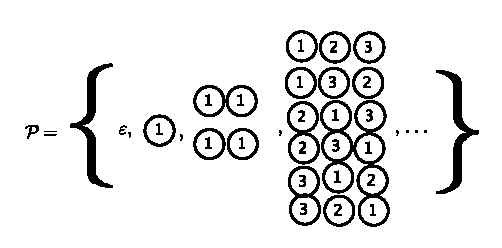
\includegraphics[width=.5\textwidth]{permutation.eps}
	\caption{Класс перестановок}
	\label{fig:permutation}	
\end{figure}

Экспоненциальная производящая функция для класса перестановок имеет вид
\[
	P(z) = \sum_{n \geq 0} n! \dfrac{z^n}{n!} = \sum_{n \geq 0}z^n = 
	\dfrac{1}{1 - z} \enspace .
\]

Заметим, что перестановка~--- это \textit{последовательность атомов}, то есть 
\textsc{seq}(\( \bullet \)), и производящая функции одного атома имеет вид \( 
\bullet(z) = z \).
\end{example}

\begin{example}[Множества]
	Количество способов составить множество из \( n \) атомов равно \( 1 \). Мы 
	ведь договорились, что атомы это последовательные натуральные числа от \( 1 
	\) до \( n \). Значит, экспоненциальная производящая функция для класса 
	множеств имеет вид
	\[
		S(x) = 1 + \dfrac{1}{1!}x + \dfrac{1}{2!}x^2 + \ldots = e^x
	\]
\end{example}

\begin{example}[Циклические графы]
	Рассмотрим циклические перестановки \( n \) объектов. Количество 
	циклических перестановок равно \( (n-1)! \): циклическая перестановка 
	определяется последовательностью элементов, которые идут после <<1>>, а 
	следовательно, образует перестановку \( (n-1) \) элемента.
	
	Значит, экспоненциальная производящая функция циклических графов имеет вид
	\[
		C(z) = \sum_{n \geq 0} (n-1)! \dfrac{z^n}{n!} = \sum_{n \geq 1} 
		\dfrac{z^n}{n} = \log \dfrac{1}{1 - z} \enspace .
	\]
\end{example}

При этом чтобы найти количество \textit{различных} объектов из \( n \) атомов, 
нужно определить, какие структуры мы считаем \textit{изоморфными}. Другими 
словами, как только мы определяем \textit{правило} \( F \), которое каждой 
биекции \( U 
\to V \) сопоставляет транспорт \( \gamma \to \beta \), то мы получаем 
помеченный класс объектов, который порождается этим правилом. Скажем, 
если в 
указанном дереве переставить в любом порядке вершины \( b, e, f \), то 
структура \( \gamma \) останется неизменной, значит, это одна и та же 
структура. Но если поменять местами вершины \( d, a \), то структура будет 
другая.

\begin{example}[Снова бюллетени]
Как и было обещано, вернёмся к бюллетеням с различимыми кандидатами. Снова 
попробуем получить выражение для экспоненциальной производящей функции для 
одного \textit{уровня}, забыв про бюллетени. На этот 
раз \textit{уровень}~--- это всё ещё \textit{множество} <<атомов>> 
(кандидатов), и количество уровней с \( n \) атомами всё ещё равно \( 1 \) 
(потому что такой уровень имеет вид множества \( \{1, 2, \ldots, n\} \)). Таким 
образом, экспоненциальная производящая функция для уровня имеет вид
\[
	\mathrm{Level} (x) = \dfrac{1}{1!} x + \dfrac{1}{2!} x^2 + \dfrac{1}{3!}x^3 
	+ \ldots = e^x - 1
	\enspace .
\]
Мы вычитаем единицу потому что пустой уровень запрещён.
Попробуем составить бюллетень из двух уровней. Если в таком бюллетене 
содержится \( n \) кандидатов, то на первом уровне их \( j \), а на втором \( 
n-j \). При этом кандидатам первого уровня необходимо раздать какие-то номера 
из множества \( \{1, 2, \ldots, n\} \), а кандидатам второго уровня~--- \( 
(n-j) \) оставшихся. Количество способов выбрать эти номера равно \( {n \choose 
j} = \dfrac{n!}{j! (n-j)!} \). Суммируя по всем \( j \), получаем выражение для 
числа двухуровневых бюллетеней с \( n \) кандидатами:
\[
	c_n = \sum_{j=0}^{n} {n \choose j} a_j a_{n-j} \enspace ,
\]
где \( a_j \)~--- количество одноуровневых бюллетеней с \( j \) кандидатами. С 
другой стороны, можно заметить, что произведение двух формальных степенных 
рядов типа экспоненциальной производящей функции, имеет вид
\begin{multline*}
	\left( a_0 + \dfrac{a_1}{1!}x + \dfrac{a_2}{2!}x^2 + \ldots
    \right )
	\left( b_0 + \dfrac{b_1}{1!}x + \dfrac{b_2}{2!}x^2 + \ldots
    \right)
	= \\
	a_0 b_0 + \dfrac{a_0 b_1 + a_1 b_0}{0!1!} x + 
	\left(\dfrac{a_0 b_2}{0!2!} + \dfrac{a_1b_1}{1!1!} + \dfrac{a_2 
	b_0}{2!0!}\right)x^2 + \ldots
\end{multline*}
То есть коэффициент при \( x^n \) равен
\[
	\sum_{j \geq 0} \dfrac{a_j b_{n-j}}{j! (n-j)!} = \dfrac{1}{n!} c_n
	\enspace .
\]
По аналогии, составляются не только двойки, но и тройки, четвёрки, кортежи 
длины \( k \). Объединяя бюллетени со всевозможным числом уровней \( k \), 
получаем
\[
	\mathrm{Ballot}(x) = \sum_{k \geq 1} \mathrm{Level}^{[k]}(x) = \sum_{k \geq 
	1} (e^{x} - 1)^k = \dfrac{1}{2 - e^x} \enspace .
\]
Давайте забежим вперёд оценим асимптотику роста коэффициентов \( b_n \) с 
помощью методов ТФКП. Вообще в этом семинаре я хотел бы сделать упор на 
комбинаторную природу, а не на аналитическую, поэтому в первом чтении этот 
фрагмент можно пропустить.

Оказывается, можно получить явную формулу в виде бесконечной суммы с помощью 
разложения
\[
	\mathrm{Ballot}(z) = \dfrac{1}{2} \dfrac{1}{1 - \tfrac12 e^{z}} = 
	\sum_{\ell \geq 0} 
	\dfrac{1}{2^{\ell + 1}} e^{\ell z} \enspace ,
\]
откуда \( R_n = \dfrac{1}{2} \sum_{\ell = 0}^{\infty} \tfrac{\ell^n}{2^\ell} 
\). Эта формула довольно милая, но нас интересует скорее асимптотика в главном 
члене. Поэтому мы пойдём другим путём.

Если рассматривать функцию \( f(z) = \dfrac{1}{2 - e^z} \) как функцию 
комплексного переменного, то она обращается в бесконечность (ещё говорят, что у 
неё есть полюса) в точках \( e^z = 2 \), что эквивалентно
\[
	z_k = \log 2 + 2 \pi i k, \quad k \in \Z \enspace .
\]
Ближайший к нулю полюс находится в точке \( z_0 \log 2 \approx 0.69314 \). В 
окрестности точки \( z_0 \) мы имеем \( f(z) \sim -\dfrac12 \cdot \dfrac{1}{z - 
\log 
2}\), ещё говорят, что это \textit{полюс первого порядка}. Чуть позже мы 
докажем \textit{теорему}, которая гласит, что из асимптотической 
эквивалентности функций следует асимптотическая эквивалентность коэффициентов 
их степенных рядов. Более строго теорема формулируется так:

\begin{theorem}[{\cite[Theorem IV.10, page 258]{ac}}]
	Пусть \( f(z) \colon \C \to \C \)~--- функция, \textit{мероморфная} во всех 
	точках диска \( |z| \leq R \) (мероморфная означает, что все особенности 
	имеют тип полюсов), и имеет полюс в точке \( z = \alpha \), \( 0 < |\alpha| 
	< R 
	\). Тогда существует многочлен \( P(n) \), такой, что
	\[
		f_n = [z^n] f(z) = P(n) \alpha^{-n} + O(R^{-n}) \enspace .
	\]
	Теорему можно обобщить на случай \( m \) полюсов и получить полное 
	асимптотическое разложение.
\end{theorem}
Применяя теорему, получаем
\[
	\dfrac{R_n}{n!} \sim \dfrac12 \left(\dfrac{1}{\log 2}\right)^{n+1} + 
	O(6^{-n}) 
	\enspace .
\]
\end{example}

% \begin{center}
% 	\underline{\textbf{Здесь заканчивается материал, который мы обсудили 
% 	2.09.2016. Дальше можно не читать.}}
% 	
% 	\underline{\textbf{Задачи можно найти в конце документа.}}
% \end{center}
% 
% \section{Композиция}
% 
% Снова порефлексируем над предыдущими примерами. Можно заметить, что для 
% экспоненциальных произвозящих функций можно определить уже больше операторов: 
% \textsc{seq}, \textsc{set}, \textsc{cyc}. При этом несложно показать, как 
% действуют эти операторы на экспоненциальных производящих функциях:
% \begin{eqnarray*}
% 	\text{\textsc{seq}}(A) &\to& \dfrac{1}{1 - A(x)} \\
% 	\text{\textsc{set}}(A) &\to& e^{A(x)} \\
% 	\text{\textsc{cyc}}(A) &\to& \log \dfrac{1}{1 - A(x)} \\	
% \end{eqnarray*}
% Докажем, например, второе свойство. Произвольные множества, составленные из 
% объектов \( \mathcal A \), можно разделить на множества из 0, 1, 2, объектов. 
% Пользуясь свойством непересекающейся суммы, можно заключить, что
% \[
% 	\text{\textsc{set}}(A) = \bigsqcup_{k \geq 0} \text{\textsc{set}}^{[k]}(A) 
% 	\enspace .
% \]
% Заметим, что каждое множество из \( k \) объектов можно сформировать как 
% последовательность из \( k \) объектов, но каждому множеству при этом будет 
% соответствовать \( k! \) различных последовательностей. Значит, производящая 
% функция для множества из \( k \) объектов равна
% \[
% 	\text{\textsc{set}}^{[k]}(A)(x) = \dfrac{A(x)^{k}}{k!} \enspace ,
% \]
% и следовательно,
% \[
% 	\text{\textsc{set}}(A)(x) = \sum_{k \geq 0} \dfrac{A(x)^{k}}{k!} = e^{A(x)} 
% 	\enspace .
% \]
% 
% Конечная цель текущего семинара -- это дать некое единое представление о 
% помеченных и непомеченных структурах. Для того, чтобы приблизиться к этому 
% представлению, нам понадобится понятие композиции\footnote{Суровая реальность такова, что до формулировки теоремы о композиции мы добрались лишь к концу третьего семинара}. Здесь дело обстоит 
% достаточно хитро: есть несколько примеров, на которых <<всё достаточно 
% понятно>>, но оказывается, что если копнуть глубже в определение, то можно 
% обнаружить для себя несколько неожиданных вещей.
% 
% \begin{definition}[{\cite[Определение 2.2.20, с.49]{gouldenjackson}}]
% 	Пусть \( \mathcal A, \mathcal B \)~--- классы комбинаторных объектов. Класс 
% 	\( \mathcal A \circ \mathcal B \) называется их \textit{композицией}, если 
% 	объекты из \( \mathcal A \circ \mathcal B \) получаются замещением 
% 	\textit{атомов} в объектах \( \mathcal A \) на объекты из \( \mathcal B \), 
% 	причём каждый элемент множества \( \mathcal A \circ \mathcal B \) можно 
% 	получить единственным способом.
% \end{definition}
% 
% \begin{example}
% 	Рассмотрим множество бинарных строк \( \mathcal S = \{0, 1\}^{\ast} = \{ 
% 	\varepsilon, 0, 1, 00, 01, 10, 11, \ldots \} \). Ясно, что количество строк 
% 	длины \( n \) равно \( 2^n \), и следовательно, производящая функция \( 
% 	S(x) \) имеет вид
% 	\[
% 		S(x) = \sum_{n \geq 0} 2^n x^n = \dfrac{1}{1 - 2x}	 \enspace .
% 	\]
% 	Заметим, что каждая строка 
% 	состоит из \textit{блоков} подряд идущих нулей и подряд идущих единиц. Если 
% 	рассмотреть множество строк, в которых нет двух подряд идущих нулей и двух 
% 	подряд идущих единиц \( \mathcal A \), то это множество устроено следующим 
% 	образом:
% 	\[
% 		\mathcal A = \{ \varepsilon, 0, 1, 01, 10, 010, 101, \ldots \}
% 	\]
% 	Его производящая функция имеет вид
% 	\[
% 		A(x) = 1 + 2x + 2x^2 + \ldots = 1 + 2\dfrac{x}{1 - x} \enspace .
% 	\]
% 	Если мы подставим вместо каждого нуля произвольное число нулей, а вместо 
% 	каждой единицы --- произвольное (ненулевое) число единиц, то композиция 
% 	соответствующих производящих функций будет иметь вид
% 	\[
% 		A\left( \dfrac{x}{1 - x}\right) = 1 + \dfrac{2\dfrac{x}{1- x}}{1 - 
% 		\dfrac{x}{1 - x}} = 1 + \dfrac{2x}{1 - 2x} = \dfrac{1}{1 - 2x} \enspace 
% 		.
% 	\]
% \end{example}
% 
% Вариация на тему этой задачи есть в упражнениях: можно будет рассмотреть 
% производящую функцию от двух переменных, и посмотреть на композицию немного с 
% другой стороны.
% 
% Не всегда получается так, что каждый объект из \( \mathcal A \circ \mathcal B 
% \) представляется 
% \textit{единственным образом} как замещение атомов объектов в \( \mathcal A \). 
% Для помеченных объектов, впрочем, это всегда так. Ради непомеченных объектов  
% приходится вводить другое определение.
% 
% \begin{definition}[{\cite[p.43]{species}}]
% 	Пусть заданы классы объектов \( \mathcal A \), \( \mathcal B \), такие, что 
% 	\( \mathcal A \) не содержит \textit{пустого объекта} (то есть, для 
% 	которого 
% 	\( U = \varnothing \)). 
% 	
% 	 Тогда их \textit{композиция} (partitional composition) это класс объектов, 
% 	 где 
% 	 структура на \( U \) являет собой тройку \( (\pi, \varphi, \gamma) \), где
% 	\begin{enumerate}
% 		\item \( \pi \)~--- разбиение \( U \)
% 		\item \( \varphi \) является \( \mathcal A \)-структурой над классами 
% 		\( \pi \)
% 		\item \( \gamma = (\gamma_p)_{p \in \pi} \)~--- набор \( 
% 		\mathcal B \)-структур внутри каждого класса \( p \in \pi \).
% 	\end{enumerate}
% \end{definition}
% 
% Это определение гораздо лучше, потому что оно корректно задаёт композицию для 
% любых двух классов \( \mathcal A \), \( \mathcal B \). Его единственный 
% недостаток состоит в том, что с новым определение композиции, соответствующее 
% равенство композиций производящих функций уже не выполнено:
% \[
% 	F \circ G(x) \neq F(G(x)) \enspace .
% \]
% 
% \section{Цикловой индекс}
% 
% Цикловой индекс --- это формальный степенной ряд, зависящий от есконечного 
% количества переменных, но при этом каждое его слагаемое зависит лишь от 
% конечного набор аргументов. До конца этого семинара будет удобно придерживаться 
% следующей системы обозначений: если задан класс объектов \( F \), то его 
% экспоненциальная производящая функция будет обозначаться \( F(x) \), 
% обыкновенная производящая функция через \( \widetilde F(x) \), а цикловой 
% индекс через \( Z_F(x_1, x_2, \ldots) \).
% 
% В этом разделе проявится \textit{алгебраическая структура} перечислительной 
% комбинаторики: чтобы двигаться дальше, нам понадобятся элементы теории групп 
% (или хотя бы теории перестановок).
% 
% \begin{definition}
% 	Цикловой тип перестановки \( \sigma \) это последовательность \( \sigma_1, 
% 	\sigma_2, \ldots \), где \( \sigma_k \) равно числу циклов длины \( k \) в 
% 	разложении \( \sigma \) на непересекающиеся циклы.
% \end{definition}
% 
% \begin{definition}
% 	\textit{Цикловой индекс} класса объектов \( F \) это формальный степенной 
% 	ряд
% 	\[
% 		Z_F(x_1, x_2, x_3, \ldots) = \sum_{n \geq 0} \dfrac{1}{n!} \left(
% 			\sum_{\sigma \in S_n} \text{fix } F[\sigma] 
% 			x_1^{\sigma_1}x_2^{\sigma_2} 
% 			x_3^{\sigma_3}\cdots
% 		\right) \enspace ,
% 	\]
% 	где \( \text{fix }F[\sigma] \) это число \( F \)-структур на \( \{1, 2, 
% 	\ldots, n\} \), которые перестановка \( \sigma \) переводит в себя.
% \end{definition}
% 
% Как и всегда, чтобы понять, что кроется за этим абстрактным определением, 
% обсудим несколько примеров.
% 
% \begin{example}
% 	Рассмотрим класс \textit{инволюций} Inv (таких перестановок, которые не 
% 	имеют только циклы длины 1 и 2 в своём цикловом разложении) и перестановку 
% 	\( \sigma \) множества \( \{a,b,c,d,e\} \), заданную рисунком 
% 	\ref{fig:sigma}. Всего существует ровно 26 инволюций на 5 объектах, и 
% 	перестановка \( \sigma \) задаёт биекцию из множества инволюций в себя. 
% 	Такая перестановка имеет цикловой тип \( (2, 0, 2, 0, 0, 3) \). В 
% 	частности, \( \text{fix Inv }[\sigma] = 2 \).
% \end{example}
% 
% \begin{example}
% 	Если \( \mathcal P \)~--- класс перестановок, то цикловой индекс \( 
% 	Z_{\mathcal P} \) задаётся формулой
% 	\[
% 		Z_{\mathcal P} = \dfrac{1}{(1-x_1)(1-x_2)(1-x_3) \ldots}
% 	\]	
% \end{example}
% 
% Оказывается, понятие циклового индекса обобщает как понятие обыкновенной, так и 
% понятие экспоненциальной производящей функции.
% \begin{theorem}
% 	Для любого класса объектов \( F \) выполнено
% 	\[
% 		F(x) = Z_F(x, 0, 0, \ldots), \quad
% 		\widetilde F(x) = Z_F(x, x^2, x^3, \ldots)
% 	\]
% \end{theorem}
% 
% Доказательство этой теоремы будет упражнением. Первый случай доказывается чуть 
% проще, для второго нужно воспользоваться леммой Бёрнсайда.
% 
% \begin{example}
% 	В качестве примера можно получить производящие функции для перестановок как 
% 	помеченных и непомеченных объектов:
% 	\[
% 		P(x) = \dfrac{1}{1 - x}, \quad
% 		\widetilde P(x) = \dfrac{1}{(1 - x)(1 - x^2)(1 - x^3) \ldots}
% 	\]
% 	Нужно обратить внимание на то, что хоть \( P(x) \) имеет производящую 
% 	функцию как для последовательностей, его обыкновенная производящая функция 
% 	не равна \( \dfrac{1}{1 - x} \). Чтобы прочувствовать это различие, нужно 
% 	прочитать несколько определений на тему <<какие класс структур мы считаем 
% 	изоморфными>>. Объяснение содержится в \cite[p. 20]{species}
% \end{example}
% 
% \subsection{Лирическое отступление на тему изоформизма классов объектов}
% 
% Строго говоря, можно назвать два класса структур \textit{идентичными}, если они 
% содержат одни и те же структуры. Но тогда нам придётся считать два различных 
% способа построения корневых подвешенных деревьев различными.
% 
% Эквипотентность, в свою очередь, размывает определение различных структур. Нам 
% бы хотелось, чтобы понятие \textit{перестановки} (биекции из множества \( 
% \{1,2, \ldots, n\} \) в себя) отличалось от понятия 
% \textit{последовательности}. Мы хотим, чтобы у этих классов были разные 
% обыкновенные производящие функции. Хорошее определение изоморфизма находится 
% где-то посередине.
% 
% \begin{definition}[{\cite[Definition 12, p.21]{species}}]
% 	Пусть \( F \) и \( G \)~--- два класса объектов. Будем обозначать через \( 
% 	F[U] \) множество объектов вида \( (U, \gamma) \), которые являются 
% 	структурами над \( U \). \textit{Изоморфизмом} 
% 	между \( F \) и \( G \) называется семейство биекций \( \alpha_U \colon 
% 	F[U] \to G[U] \), для которого данная \textit{диаграмма коммутативна}:
% 	\[
% 	\begin{CD}
% 		F[U] @>{\alpha_U}>> G[U]\\
% 		@V{F[\sigma]}VV @VV{G[\sigma]}V\\
% 		F[V] @>>{\alpha_V}> G[V]
% 	\end{CD}
% 	\]
% 	Другими словами, \( \sigma \cdot \alpha_U(s) = \alpha_V(\sigma \cdot s) \) 
% 	для любого объекта \( s \in F[U] \).
% \end{definition}
% 
% Хорошая новость состоит в том, что для изоморфных структур сохраняются все три 
% типа производящих функций: если \( F \cong G \), то 
% \[
% 	Z_F(x_1, x_2, \ldots) = Z_G(x_1, x_2, \ldots) \enspace .
% \]
% 
% \subsection{Важные свойства циклового индекса}
% 
% В заключение, сформулируем свойства циклового индекса, к которым мы шли в 
% течение всего рассказа. Доказательства этих свойств будут засчитываться как 
% задачи.
% 
% \begin{enumerate}
% \item \( Z_{F \sqcup G}(x_1, x_2, \ldots) = Z_F(x_1, x_2, \ldots) + Z_G(x_1, 
% x_2, \ldots) \)
% \item \( Z_{F \times G}(x_1, x_2, \ldots) = Z_F(x_1, x_2, \ldots) \cdot 
% Z_G(x_1, x_2, \ldots) \)
% \end{enumerate}
% 
% Наконец, сформулируем результат для композиции цикловых индексов, и 
% сформулируем теорему для композиции в случае обыкновенных производящих функций.
% 
% \begin{theorem}
% 	Пусть \( F \), \( G \)~--- два класса объектов, для 
% 	которых \( G \) не содержит пустого объекта. Тогда
% 	\[
% 		Z_{F \circ G}(x_1, x_2, \ldots) = Z_F(
% 			Z_G(x_1, x_2, \ldots),
% 			Z_G(x_2, x_4, \ldots),
% 			\ldots
% 		) \enspace .
% 	\]
% 	Композиция обыкновенных производящих функций имеет вид
% 	\[
% 		\widetilde{F \circ G}(x) = Z_F(\widetilde G(x), \widetilde G(x^2), 
% 		\widetilde G(x^3), \ldots)
% 		\enspace .
% 	\]
% \end{theorem}

\section{Задачи}
            
\subsection{Задачи на понимание}
\begin{enumerate}
\item Потренируйтесь в формальном описании объектов в виде \( (U, \gamma) \), 
где \( U \)~--- данные, а \( \gamma \)~--- структура объекта. Для этого 
попробуйте рассмотреть следующие классы объектов:
\begin{enumerate}
	\item \( \mathcal D \) -- класс ориентированных графов.
	\item \( \mathfrak P \) -- класс подмножеств:
	\[
		\mathfrak P[U] = \{ S | S \subseteq U \}
	\]
	\item End -- класс эндофункций:
	\[
		End[U] = \{ \psi | \psi \colon U \to U \}
	\]
\end{enumerate}
\item Докажите формулу для оператора \( \textsc{cyc} \) для экспоненциальных 
производящих функций.
\item Почему нельзя получить формулу для оператора \textsc{set} в случае 
непомеченных объектов для обыкновенных производящих функций, по аналогии с 
оператором \textsc{set} для экспоненциальных производящих функций?
%\item Выведите из формулы для композиции классов <<хорошую>> формулу \( 
%\widetilde F(\widetilde G)(x) = \widetilde{F \circ G}(x) \) для случая, когда 
%она работает, то есть когда каждый объект из класса \( F \circ G \) получается 
%единственным образом.
\end{enumerate}

\subsection{Задачи для сдачи}
\begin{enumerate}
\item(2 очка) Покажите, что обыкновенная производящая функция \( A(x) = a_0 + 
a_1 x + a_2 x^2 + \ldots \) и экспоненциальная \( E(z) = a_0 + \dfrac{a_1}{1!}z 
+ \dfrac{a_2}{2!}z^2 + \ldots \) связаны соотношением
\[
	A(x) = \int_{0}^{\infty} e^{-z} E(xz) dz
\]
\item(2 очка) Пусть Cha~--- класс неориентированных 
цепочек (последовательность атомов, которая по определению изоморфна той же 
последовательности, прочитанной справа налево). Рассмотрим следующие классы \( 
\mathbf{1} 
\)~--- класс, в котором содержится один <<пустой>> элемент без атомов, а также 
класс \( X \), который состоит ровно из одного объекта, состоящего из одного 
атома. Рассмотрим также
оператор \( E_2(\mathcal A) \), который обозначает множества из двух объектов 
\( a, b \in \mathcal A \). Докажите, что класс Cha может быть представлен в виде
\[
	\mathrm{Cha} = (\mathbf{1} \sqcup X) \times \left(\mathbf{1} \sqcup 
	\bigsqcup_{n \geq 1} 
	E_2(X^n)\right)
\]
\item(1 очко) Покажите, что класс \( \mathfrak P \) подмножеств \( \mathfrak 
P[U] = \{ S | S \subseteq U \} \) изоморфен классу \( E \times E \), где \( E 
\)~--- класс \textit{множеств}.
\item(1 очко) Рассмотрим множество бинарных строк, то есть строк из нулей и 
единиц: \( S = \{0, 1\}^{\ast} \). Рассмотрим производящую функцию \textit{от 
двух переменных}
\[
	F(x, y) = \sum_{i, j \geq 0} c_{ij} x^i y^j \enspace ,
\]
где коэффициент при \( x^i y^j \) равен количеству строк, содержащих \( i \) 
нулей и \( j \) единиц. Рассмотрим множество строк \( A \), которые не содержат 
двух подряд идущих нулей. Если взять множество таких строк, и вместо каждого 
нуля подставить непустую последовательность нулей, то можно получить множество 
всех бинарных строк. Таким образом, если мы верим в правило композиции, то
\[
	F(x, y) = A\left(\dfrac{x}{1-x}, y\right ) \enspace .
\]
Получите отсюда производящую функцию \( A(x, y) \). Затем используя это 
выражение, найдите количество строк длины \( n \), в которых нет двух подряд 
идущих нулей.
\item(1 балл) \textbf{Комбинаторные паровозики.} Рассмотрим класс 
\textit{помеченных паровозиков}, заданный системой уравнений
\[
	\begin{cases}
		Tr & =  Wa \times \text{\textsc{seq}}(Wa \times 
		\text{\textsc{set}}(Pa))\ ,\\
		Wa & = \text{\textsc{seq}}_{\geq 1}(Pl)\ ,\\
		Pl & = \bullet \times \bullet \times (1 \sqcup 
		\text{\textsc{cyc}}(\bullet) ) \ , \\
		Pa & = \text{\textsc{cyc}}(\bullet) \times \text{\textsc{cyc}}(\bullet) 
		\ .
	\end{cases}
\]
Фигурально выражаясь, \textit{паровозик} (\( Tr \)) состоит из первого 
\textit{вагона} (\( Wa \)), к которому прикреплена последовательность 
пассажирских вагонов, каждый из которых может перевозить последовательность 
\textit{пассажиров} (\( Pa \)). Сам по себе вагон состоит из 
\textit{вертикальных секций} (\( Pl \)), где у каждой секции имеется выделенный 
верх и низ, и опционально можно прикрутить \textit{колесо} (\textsc{cyc}(\( 
\bullet \))). Пассажир состоит из головы и животика, которые являются 
циклической последовательностью атомов. На рисунке \ref{fig:train} изображен 
случайный 
паровозик.

Найдите экспоненциальную производящую функцию для числа помеченных паровозиков.
\begin{figure}[h]
\centering
	\includegraphics[natwidth=811,natheight=349,width=0.8\textwidth]{train.png}
	\caption{Случайный паровозик}
	\label{fig:train}	
\end{figure}
\item(2 очка) Пусть \( \mathcal M = \text{\textsc{mset}}(\mathcal C) \), \( 
\mathcal P = \text{\textsc{pset}}(\mathcal C) \). Докажите, что
\[
	M(z) = P(z) M(z^2) \enspace .
\]
Если вы в этой задаче собираетесь воспользоваться формулами для \textsc{pset} и \textsc{mset}, то их необходимо сначала доказать. Можно не пользоваться этими формулами, и решить задачу, исходя из комбинаторных соображений.
\item(2 очка) Докажите, что количество разбиений натурального числа \( n \) в 
виде суммы множества \textit{различных} слагаемых равно количеству 
разбиений в сумму множества \textit{нечётных} (не обязательно 
различных) слагаемых. Для этого предъявите производящие функции для каждого из 
этих разбиений, и докажите, что они равны. (Другие комбинаторные доказательства 
не принимаются).
\item(2+2+2 очка) Первые три задачи, приведенные на первой странице этого 
документа, тоже можно сдавать. Каждая задача стоит 2 очка.
\item(3 очка) Пусть $n \in \mathbb N$~--- некоторое натуральное число. 
Предположим, что

\begin{tabular}{cc}
  $x + 2y = n$ & имеет $R_1$ решений в $\mathbb N_0^2$ \\
  $2x + 3y = n-1$ & имеет $R_2$ решений в $\mathbb N_0^2$ \\
  $\hdots$ & $\hdots$ \\
  $nx + (n+1)y = 1$ & имеет $R_n$ решений в $\mathbb N_0^2$ \\
  $(n+1)x + (n+2)y = 0$ & имеет $R_{n+1}$ решений в $\mathbb N_0^2$ \\
\end{tabular}

Докажите, что $\sum_{k} R_k = n+1$.
\item(2 очка) (\textbf{Численный сюрприз}). Рассмотрим константу
\[
	\varphi = \dfrac{9}{10} \cdot \dfrac{99}{100} \cdot
	\dfrac{999}{1000} \cdot \ldots
	\enspace .
\]
Удивительно, но десятичная запись этой константы имеет вид
\[
	\varphi = 0.8900100999989990000001000099999999899999000000000010 \ldots
	 \enspace .
\]
Верно ли, что десятичная запись содержит только цифры \( 0, 1, 8, 9 \)? Если 
да, то почему?

\textbf{Подсказка.} Ознакомьтесь с содержанием второго семинара, там есть теорема, которая может сильно помочь в решении данной задачи.
\item(3 очка) Обозначим через \( S_n(2) \) количество симметрических матриц \( 
n \times n \) 
с 
элементами из \( \{ 0,1,2,\ldots \} \), таких, что сумма чисел в каждой строке 
и в каждом столбце равна \( 2 \). Докажите, что
\[
	\sum_{n \geq 0} S_n(2) \dfrac{x^n}{n!} = (1-x)^{-1/2} \exp \left(
		\dfrac{x^2}{4} + \dfrac{x}{2(1-x)}
	\right) \enspace .
\]
\textbf{Подсказка.} Можно считать, что матрица является матрицей смежности некоторого 
графа.

%\item(2 очка) % операторы exp, cyc, ... для ogf, оператор cube
%\item(1 очко) придумайте два класса, для которых не выполнено соотношение \( 
%F\circ G(x) = F(G(x)) \) как для классов непомеченных объектов.
%\item(1 очко) Докажите первые два свойства циклового индекса (объединение и 
%декартово произведение).
%\item(3 очка) Докажите теорему о композиции для циклового индекса.
%\item(2 очка) Покажите, что цикловой индекс для бюллетеней имеет вид
%\[
%	Z_{\text{Ballot}}(x_1, x_2, \ldots) = \dfrac{1}{2 - \exp \left(
%		x_1 + \dfrac{x_2}{2} + \dfrac{x_3}{3} + \ldots
%	\right)} \enspace .
%\]
%Получите отсюда формулы для помеченных и непомеченных бюллетеней.
\end{enumerate}

\footnotesize
\bibliographystyle{plain}
\bibliography{biblio}
    
\end{document}
